\documentclass[]{BasiliskReportMemo}
\usepackage{AVS}
\usepackage{float}
\usepackage{array}

\newcommand{\submiterInstitute}{Autonomous Vehicle Simulation (AVS) Laboratory,\\ University of Colorado}

\newcommand{\ModuleName}{RadiationPressure}
\newcommand{\subject}{Radiation Pressure Model}
\newcommand{\status}{Initial document draft}
\newcommand{\preparer}{S. Carnahan}
\newcommand{\summary}{The radiation pressure module is responsible for calculating the dyamic effects of radiation pressure on a spacecraft. Effects can be calculated either by use of a simplified ``cannonball" method or table look-up. A unit test has been written which checks both calculation methods against expected output values. The code is working fully and providing accurate results.}
\newcommand{\testname}{test\_radiationPressure.py }


\begin{document}


\makeCover


%
%	enter the revision documentation here
%	to add more lines, copy the table entry and the \hline, and paste after the current entry.
%
\pagestyle{empty}
{\renewcommand{\arraystretch}{1.1}
\noindent
\begin{longtable}{|p{0.5in}|p{4.5in}|p{1.14in}|}
\hline
{\bfseries Rev}: & {\bfseries Change Description} & {\bfseries By} \\
\hline
Draft & Initial document creation & \preparer\\
\hline

\end{longtable}
}

\newpage
\setcounter{page}{1}
\pagestyle{fancy}

\tableofcontents
~\\ \hrule ~\\

	\section*{Nomenclature\\}
	\noindent\begin{tabular}{@{}lcl@{}}
	$AU$ &=& 1 astronomical unit \\
	${SF}_{AU}$ &=& average solar flux at 1 AU from the sun \\
	${SF}_{\mathrm{eff}}$ &=& effective solar flux at 1 AU given eclipse conditions \\
	$F_{SF}$ &=& solar factor (between 0 and 1) applied to the solar flux due to an eclipse\\
	$p_{SR}$ &=& pressure due to solar radiation\\
	$c$  &=&  speed of light\\
	$\mathbf{F}_{\mathrm{radiation}}$  &=&  Force vector on spacecraft due to solar radiation\\
	$c_{R}$ &=& coefficient of reflectivity (between 0 and 2)\\
	$A_{\odot}$ &=& equivalent cross sectional area of the spacecraft as seen by solar radiation pressure \\
	$\mathbf{r}_{\mathrm{sun}}$ &=& position vector from the spacecraft to the sun in the spacecraft body frame \\
	
\end{tabular} 

\pagebreak

\section{Introduction}
The Basilisk radiation pressure module (radiation\_pressure.cpp) is responsible for calculating the effects of radiation pressure on a spacecraft. A basic flow of inputs and outputs is visualized in \ref{img:codeFlow}\\

\begin{figure}[H]
\centering 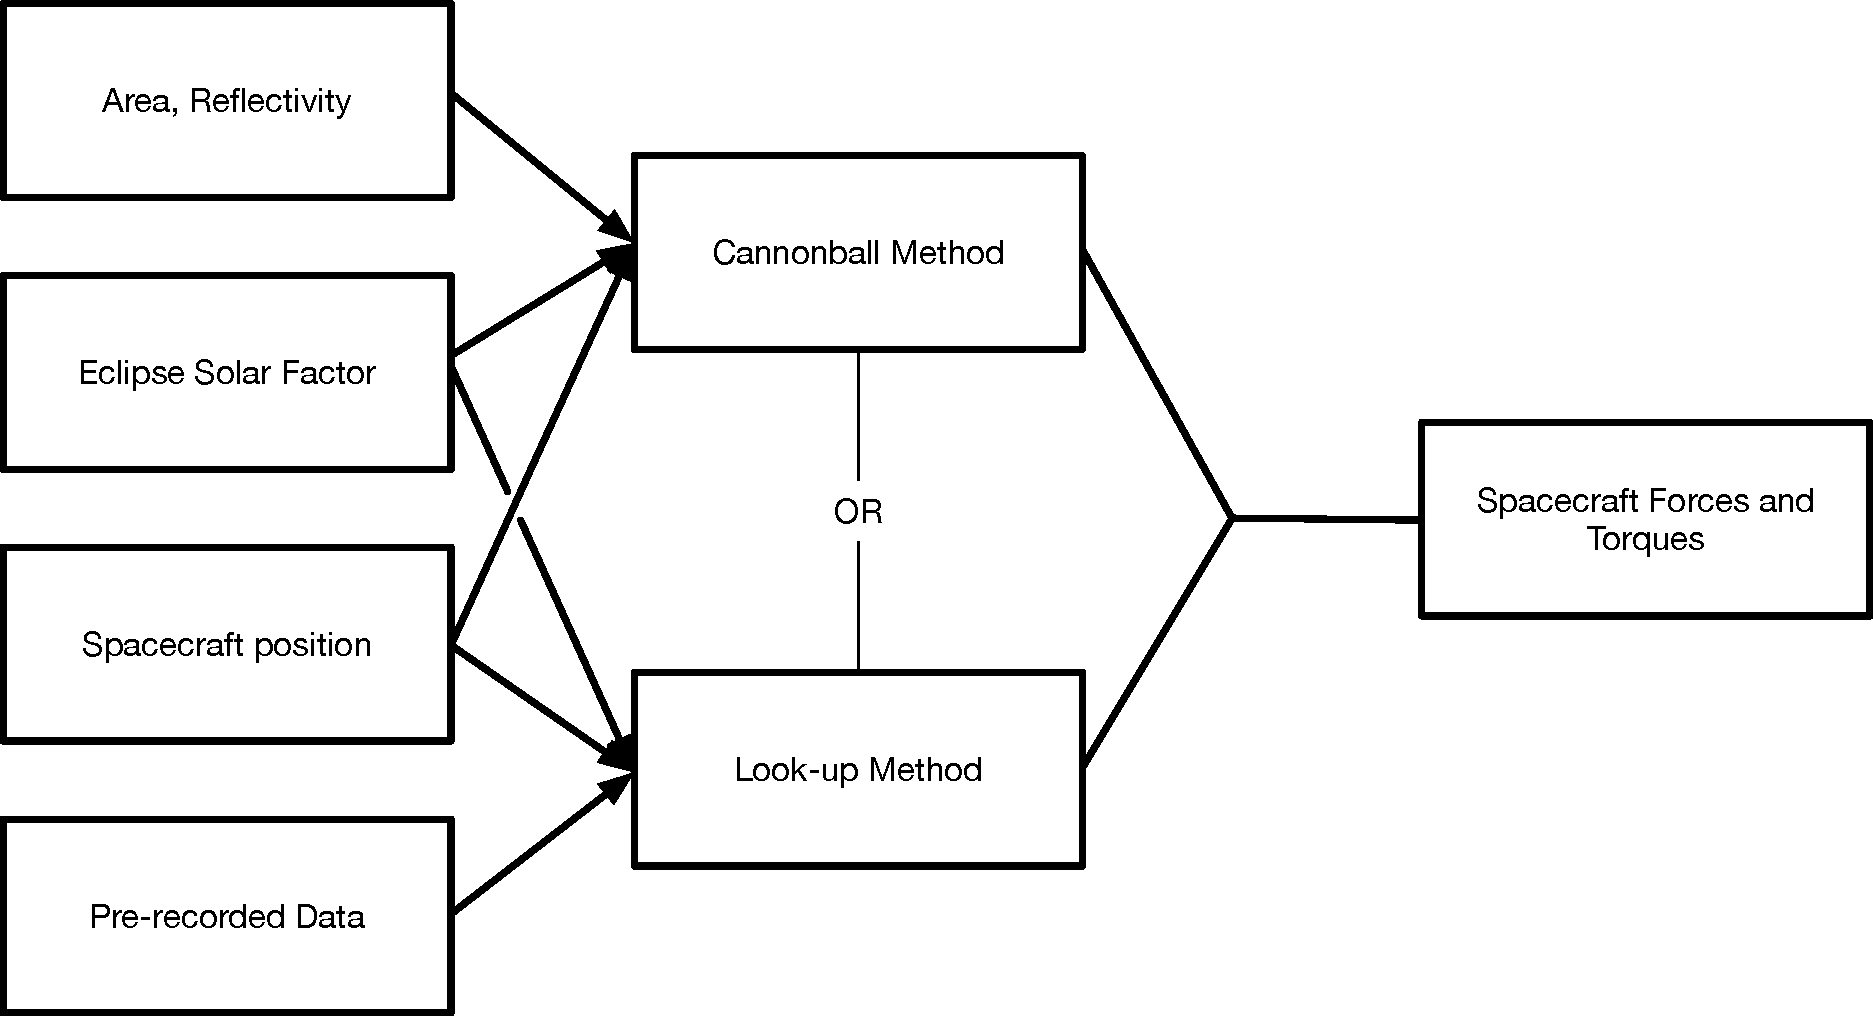
\includegraphics[height=0.5\textwidth, keepaspectratio]{Figures/codeFlow.pdf}
\caption{Inputs necessary for solar radiation pressure calculations flow into either the cannonball method or the look-up method. These methods output their torque and force contributions to the spacecraft.}
\label{img:codeFlow}
\end{figure}

The mathematical models used are described below. The code unit tests are then presented and discussed.



\section{Mathematical Model}
Both methods of calculating solar radiation pressure have simple implementations in Basilisk using basic coefficients and assumptions. The methods of arriving at these coefficients can be complex and making the coefficients time-varying to improve accuracy can greatly increase complexity. The cannonball method used here essentially follows the mathematics described by Vallado\cite{vallado2001}.
\subsection{Radiation Model}
Radiation is modeled by using the solar flux at one astronomical unit and scaling by distance from the sun relative to 1 AU. The solar flux at one AU is taken as :
\begin{equation}
SF_{AU} = 1372.5398    [W/m^2]
\end{equation}
\subsubsection{Solar Eclipses}
Solar eclipses are are detected by the basilisk eclipse module. The effects of the eclipse are calculated into a solar factor which is applied to the solar flux to create an effective solar flux. 
\begin{equation}
SF_{\mathrm{eff}} = F_{SF} (SF_{AU})
\end{equation}
Then, calculations are carried on as seen below.

\subsection{Radiation Pressure Model}
\subsubsection{Cannonball Method}
The radiation pressure at 1AU, $p_{SR}$, can be taken as the solar flux divided by the speed of light. 
\begin{equation}
p_{SR} = \frac{SF_{\mathrm{eff}}}{c}
\end{equation}
Then, a ``scaling factor'' can be determined. This ``scaling factor" is equivalent to the magnitude of the solar radiation force divided by the distance between the spacecraft and the sun:
\begin{equation}
\frac{|\mathbf{F}_{\textrm{radiation}}|}{|\mathbf{r}_{\textrm{sun}}|} = \frac{-c_{R}p_{SR}A_{\odot}{AU}^2}{c |\mathbf{r}_{\textrm{sun}}|^3}
\end{equation}
This factor is then multiplied by the position vector from the spacecraft to the sun to get the force on the spacecraft due to solar radiation pressure.
\begin{equation}
{\mathbf{F}_{\textrm{radiation}}} = \frac{|\mathbf{F}_{\textrm{radiation}}|}{|\mathbf{r}_{\textrm{sun}}|}  \mathbf{r}_{\textrm{sun}}
\end{equation}
The user must provide the coefficient of reflection and the equivalent area of the spacecraft to use this method.\\
\subsubsection{Table Look-up Method}
For the table look-up method, pre-determined values of torque and force acting on the spacecraft due to radiation pressure are given. It is required that these values be given at 1AU from the sun and with a corresponding direction vector form the spacecraft to the sun.\\\\
The look-up works by finding the direction vector in the given tables which most closely matches the spacecraft's current position vector. Then, the corresponding force and torque values are taken from the table and scaled according to the magnitude of the spacecraft-sun position vector.\\\\
Most important to the user of the table look-up method is the required input and format of data. Data must be recorded in XML format. As an example, see ../cube\_lookup.xml (in the radiation pressure folder). Additionally, a utility script called parseSRPLookup.py is provided there to read the XML input into numpy arrays. Experienced users are welcome to store their data in their own format and load it into equivalent numpy arrays as they see fit.\\\\
An example of using the provided python script to load data is shown in \testname. Note that this also requires import of the unitTestSupport library.\\
\subsection{Variable Definitions}
The variables in Table \ref{tabular:vars} are available for user input. Variables used by the module but not available to the user are not mentioned here. Variables with default settings do not necessarily need to be changed by the user, but may be.
	\begin{table}[H]
		\caption{Definition and Explanation of Variables Used.}
		\label{tab:errortol}
		\centering \fontsize{10}{10}\selectfont
		\begin{tabular}{ | m{3cm}| m{3cm} | m{3cm} | m{6cm} |} % Column formatting, 
			\hline
			\textbf{Variable}   		& \textbf{LaTeX Equivalent} 	&		\textbf{Variable Type} & \textbf{Notes} \\ \hline
			stateInMsgName			&N/A		   							    & string 								& Default setting: ``inertial\_state\_output". This is the message from which the radiation pressure module receives spacecraft inertial data.\\ \hline
			sunEphmInMsgName	& N/A 										& string 								& Default setting: ``sun\_planet\_data". This is the message through which radiation pressure gets information about the sun and planets.\\ \hline
			area 						  	  & $A_{\odot}$							    & double 								& [m2] Default setting: 0.0f. Required input for cannonball method to get any real output. This is the area to use when approximating the surface area of the spacecraft.\\ \hline
			coefficientReflection 	  & $c_{R}$ 								& double 								& Default setting: 1.2. This is a factor applied to the radiation pressure based on spacecraft surface properties.\\ \hline
			useCannonballModel	   & N/A 									   & bool 									& Default setting: True. To switch cannonball mode off, use the call setUseCanonballModel(``False")\\ \hline
		\end{tabular}
	\label{tabular:vars}
	\end{table}
\section{Library}
This section means nothing to me.

\section{Unit Test}

This test is located at {\tt SimCode/dynamics/RadiationPressure/\_UnitTest/\testname} In order to get good coverage of all the aspects of the module, the test is broken up into two sub-tests. In each sub-test, a spacecraft is placed in the solar system and acted upon by the Sun. \par

\subsection{``Cannonball" Method} This test utilizes the ``cannonball" method to calculate the effects of radiation pressure on spacecraft dynamics. The cannonball method approximates the spacecraft as a sphere. External forces in the inertial and body frame, as well as external torques in the body frame, are checked against known values.
\subsection{Table Look-up Method} This test uses a stored table of known effects of radiation pressure. It looks up values and compares them to the expected result to validate radiation pressure table look-up capabilities.


\subsection{Test Parameters}

This section summarizes the error tolerances for each test. Error tolerances are determined based on whether the test results comparison should be exact or approximate due to integration or other reasons. Error tolerances for each test are summarized in table \ref{tab:errortol}. 

\begin{table}[htbp]
	\caption{Error tolerance for each test.}
	\label{tab:errortol}
	\centering \fontsize{10}{10}\selectfont
	\begin{tabular}{ c | c } % Column formatting, 
		\hline
		\textbf{Test}   							& \textbf{Tolerated Error} 						  \\ \hline
		``Cannonball" &\input{AutoTex/cannonballAccuracy}		   \\ \hline
		Look-up					& \input{AutoTex/lookupAccuracy}														   \\ \hline
	\end{tabular}
\end{table}


\subsection{Test Results}

All checks within \testname passed as expected. Table \ref{tab:results} shows the test results.

\begin{table}[htbp]
	\caption{Test results.}
	\label{tab:results}
	\centering \fontsize{10}{10}\selectfont
	\begin{tabular}{c | c | c  } % Column formatting, 
		\hline
		\textbf{Test} 				      & \textbf{Pass/Fail} 						   		   & \textbf{Notes} 									\\ \hline
		``Cannonball"	   			  	&\input{AutoTex/cannonballPassFail}      &\input{AutoTex/cannonballFailMsg} 	 \\ \hline
		Look-up	   	                     &\input{AutoTex/lookupPassFail}              &\input{AutoTex/lookupFailMsg}            \\ \hline
	\end{tabular}
\end{table}

\subsection{Test Coverage}
The test covers 2000\% of the code.
\section{Conclusion}
What a great piece of code.

\bibliography{bibliography}{}
\bibliographystyle{plain}

\end{document}
